%%%%%%%%%%%%%%%%%%%%%%%%%%%%%%%%%%%%%%%%%%%%%
\section{The rate of phase space mixing}
\label{Sec:Rates}
%%%%%%%%%%%%%%%%%%%%%%%%%%%%%%%%%%%%%%%%%%%%%

In this section we analyze how fast the clouds which relax mix, and how fast the potential which they generate approaches a stationary profile, as functions of their mass and of the dependence of their DF on the action variable. In the absence of self-gravity the rate is set by the behavior of the DF at the edges of its support, Eq.~(\ref{Eq:Tail}). We find that self-gravity slows down the mixing of all the clouds whose DF is smooth, and that the decay remains algebraic, with an exponent which changes continuously with the mass and depends on the shape of the cloud. The reason is twofold. During the first units of $\tau_1$ the gas which is transported towards the circular orbit lowers the regularity of the DF at the inner edge of its support, which sets a slower tail. Afterwards, the part of the DF which is not yet mixed acts through its potential on the mixed part, and the linear response of the latter, which is concentrated at the edges of its support, slows down the mixing further; at late times this response is damped by the smoothing of the abrupt edges of the mixed state. That self-gravity delays the phase mixing of a perturbation has also been found for the motion of the stars perpendicular to the plane of a galactic disk~\cite{kDlW19,lW23,tAtA26}.
\EJ{Placed after section~\ref{Sec:FarFromEq} as in the scheme of 16 November. For now it uses the parameter $\Gamma$ and the shapes of section~\ref{Sec:Epicyclic}; in the reorganization $\Gamma$ moves to section~\ref{SubSec:FarRuns}.}


\subsection{Simulations}
\label{SubSec:RatesRuns}

Since the decay of $h_n$ is algebraic, its exponent can only be measured if the simulations resolve small values of $|h_n|$ over many units of $\tau_1$. For this purpose we have carried out the simulations listed in Table~\ref{Tab:Rates} on a lattice with $N_J\times N_Q = 3200\times 100$ points, without the points whose weight is smaller than $10^{-7}$ of the largest one. They comprise the reference cloud of section~\ref{Sec:FarFromEq}, that is, the cloud~(\ref{Eq:Pulse}) with $\sigma_Q = \sigma_J = 0.1$ and $L_0 = 2$ in the isochrone potential, with four masses, and four of the shapes of section~\ref{SubSec:EpiProfiles} with two masses each: $J^4\exp(-J^2/\sigma_J^2)$, $(J - 0.05)_+^2\exp(-J^2/\sigma_J^2)$, the ring $\exp[-(J - 0.15)^2/0.03^2]$ and the water bag, which is constant for $0.05\leq J\leq 0.25$. We label the masses by the parameter $\Gamma$ of Eq.~(\ref{Eq:Gamma}), which compares the angular velocity of the rotation that the gas induces at its distance from the circular orbit with the one of the differential rotation of the orbits at the same distance, and which is determined by the initial datum. For the reference cloud $\Gamma = 0.025$, $0.05$, $0.1$ and $0.15$ correspond to $M_{gas}/M$ between $0.0022$ and $0.013$, that is, to $\mu$ between $0.14$ and $0.35$, and for the other shapes $\Gamma = 0.05$ and $0.1$ correspond to $M_{gas}/M$ between $0.0063$ and $0.014$. All these clouds relax: for clouds which are compact in angle and whose DF vanishes at the circular orbit, a core forms when $\Gamma$ is between $0.23$ and $0.29$ (sections~\ref{Sec:FarFromEq} and~\ref{SubSec:EpiProfiles}).

These simulations have been carried out with the second implementation of the PIC method described in section~\ref{SubSec:DistRuns}, with all the gas particles at $L = L_0$, with $\Delta t = 0.05$ and the grid spacing $\Delta r = 0.1$, and they extend over $30\tau_1$, with $\tau_1 = 327$, $324$, $392$, $702$ and $451$ for the reference cloud and the shapes in the order given above. The observables are computed with the action-angle variables of the instantaneous potential. In order to test the convergence, we have repeated the simulation of the reference cloud with $\Gamma = 0.1$ on a lattice with $6400\times 200$ points. Over $3\leq t/\tau_1\leq 20$ the envelopes of $|h_1|$, $|h_2|$, $|h_3|$ and of the deviation~(\ref{Eq:deltaPhiNorm}) of the potential of the gas differ from those on the coarser lattice by at most $0.1$, $2.2$, $5.1$ and $1.4$ percent, respectively, and the envelope of $|h_1|$ differs by at most $3.9$ percent up to $t = 30\tau_1$. Beyond $t = 20\tau_1$ the higher harmonics and the potential depend on the lattice, and we do not use them. On the lattices of section~\ref{Sec:FarFromEq}, by contrast, the higher harmonics are dominated by the discreteness of the particles from $t\approx 8\tau_1$ on. In particular, the mean values of $|h_1|/h_0$ over $10\leq t/\tau_1\leq 20$ quoted in section~\ref{Sec:FarFromEq} measure a tail which continues to decay, not a level at which the mixing stops.\EJ{To be adjusted in the wording of section~\ref{SubSec:FarRegimes} (``the level which is reached at late times'').}

\begin{table}[htp]
\begin{center}
\begin{tabular}{ll|c|cc|cc|c|c|c}
\hline\hline
 & & & \multicolumn{2}{c|}{slope of $|h_1|$} & \multicolumn{2}{c|}{slope of $\|\delta\Phi\|$} & $|h_1|/h_0$ & & \\
dependence on $J$ & $\Gamma$ & $M_{gas}/M$ & $3$--$10$ & $10$--$20$ & $3$--$10$ & $10$--$20$ & at $20\tau_1$ & $q_1$ & $J_{in}/\sigma_J$ \\
\hline
\TabColas
\hline\hline
\end{tabular}
\end{center}
\caption{Simulations of clouds which relax, on the lattice with $3200\times 100$ points, and exact solutions in the absence of self-gravity ($\Gamma = 0$). Slopes of the envelopes of $|h_1|/h_0$ and of the deviation $\|\delta\Phi\|$ of the potential of the gas, Eq.~(\ref{Eq:deltaPhiNorm}), as functions of $\log t$ over the intervals $3\leq t/\tau_1\leq 10$ and $10\leq t/\tau_1\leq 20$; value of $|h_1|/h_0$ at $t = 20\tau_1$; exponent $q_1$ of the first harmonic of the DF near the circular orbit at $t = 10\tau_1$ (for $\Gamma = 0$, the exponent of the initial datum); and, for the shapes whose support does not reach the circular orbit, the action $J_{in}$ beyond which the angle average of the DF exceeds one percent of its maximum at $t = 10\tau_1$ (for $\Gamma = 0$, in the initial datum). The ring is $\exp[-(J - 0.15)^2/0.03^2]$, and the water bag is constant for $0.05\leq J\leq 0.25$.}
\label{Tab:Rates}
\end{table}


\subsection{Decay of the mixing and of the potential}
\label{SubSec:RatesDecay}

\begin{figure}[htp]
\centerline{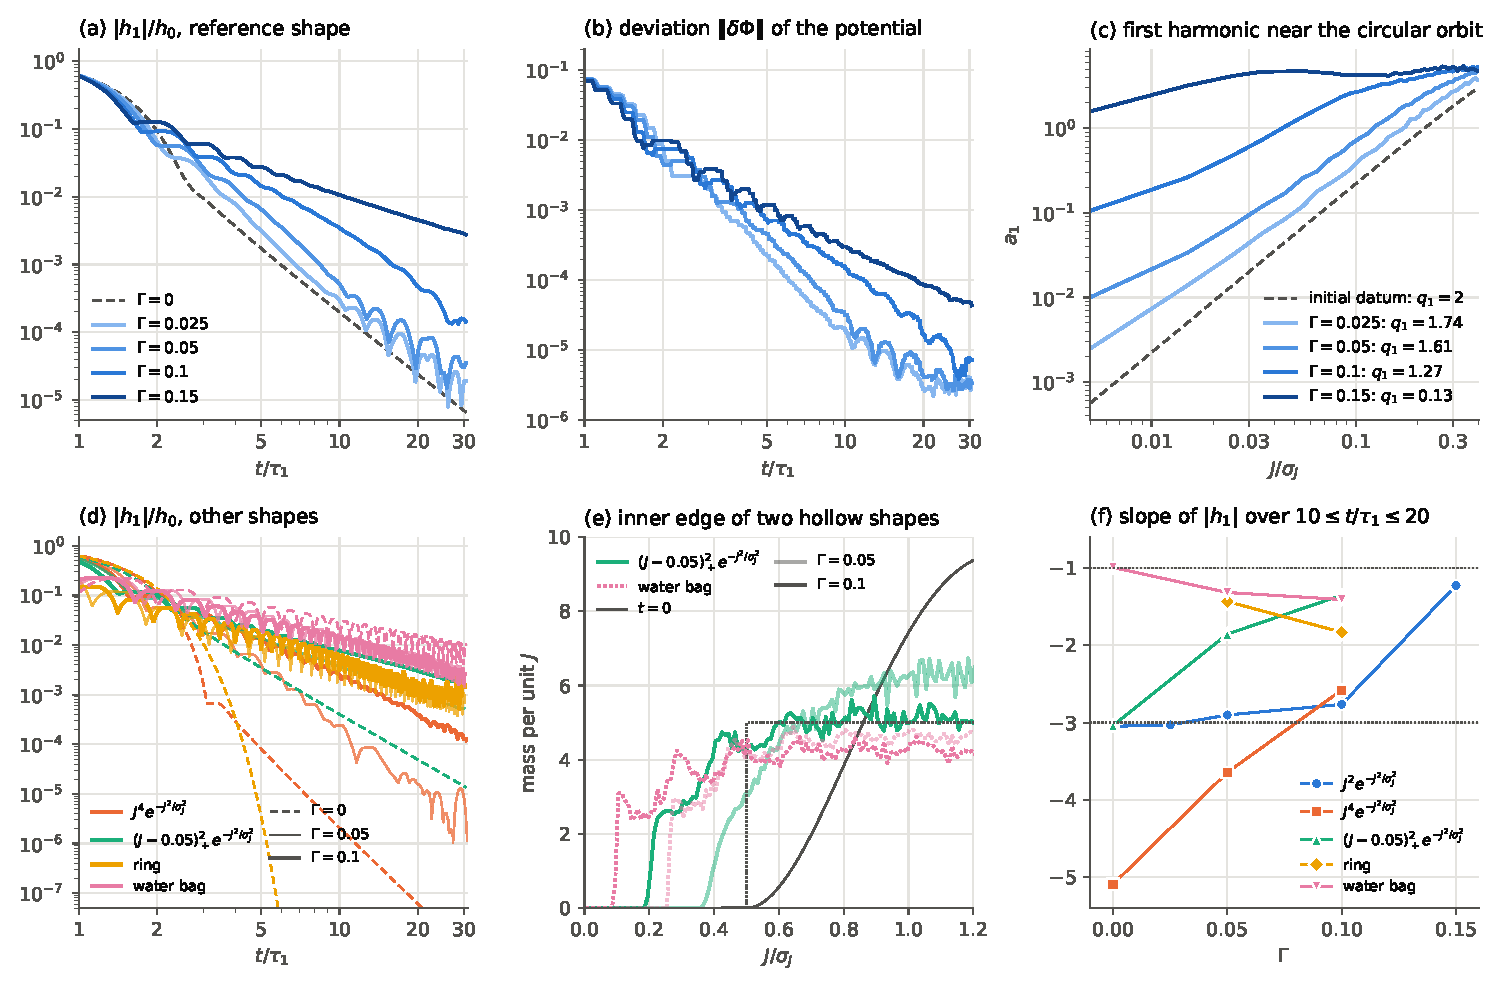
\includegraphics[width=\textwidth]{figuras/colas_alta.pdf}}
\caption{Clouds which relax, on the lattice with $3200\times 100$ points. (a) Envelope of $|h_1|/h_0$ for the reference cloud with several values of $\Gamma$; the dashed line is the exact solution in the absence of self-gravity. (b) Envelope of the deviation~(\ref{Eq:deltaPhiNorm}) of the potential of the gas for the same simulations. (c) Modulus $a_1$ of the first harmonic of the DF with respect to the angle variable near the circular orbit at $t = 10\tau_1$, per unit $J$ and per unit mass of the gas, for the same simulations, and the exponent $q_1$ of a fit $a_1\propto J^{q_1}$ over $0.01\leq J/\sigma_J\leq 0.1$; the dashed line is the initial datum. (d) Envelope of $|h_1|/h_0$ for four other shapes in the absence of self-gravity (dashed lines), and for $\Gamma = 0.05$ (thin lines) and $\Gamma = 0.1$ (thick lines). (e) Mass of the gas per unit $J$ (per unit mass of the gas) near the inner edge of the support at $t = 10\tau_1$ for two shapes whose support does not reach the circular orbit, for $\Gamma = 0.05$ (light) and $\Gamma = 0.1$ (dark), and for the initial datum (gray). (f) Slope of the envelope of $|h_1|$ as a function of $\log t$ over $10\leq t/\tau_1\leq 20$; $\Gamma = 0$ refers to the exact solution in the absence of self-gravity, which for the ring decays faster than any power of $t$. The envelopes are the largest values in a moving window of width $100$, and all quantities are computed with the action-angle variables of the instantaneous potential.}
\label{Fig:Rates}
\end{figure}

Self-gravity slows down the mixing of all the shapes whose DF vanishes smoothly at the edges of its support, and the more regular the initial DF is, the stronger the effect, see Fig.~\ref{Fig:Rates}(a,d) and Table~\ref{Tab:Rates}. In the absence of self-gravity Eq.~(\ref{Eq:hnFree}) can be evaluated exactly, and the envelope of $|h_1|$ decays like $t^{-(k+1)}$, Eq.~(\ref{Eq:Tail}), where $k$ is the exponent with which the DF vanishes at an endpoint of its support: $J = 0$ for the reference cloud ($k = 2$) and for the shape $J^4\exp(-J^2/\sigma_J^2)$ ($k = 4$), $J = 0.05$ for the shape $(J - 0.05)_+^2\exp(-J^2/\sigma_J^2)$ ($k = 2$), and both endpoints for the water bag ($k = 0$). The slopes over $10\leq t/\tau_1\leq 20$ are $-3.05$, $-5.09$, $-3.04$ and $-0.99$, respectively, whereas for the ring $|h_1|$ decays faster than any power of $t$ and $|h_1|/h_0 = 2.0\times 10^{-13}$ at $t = 20\tau_1$. With self-gravity and $\Gamma = 0.1$, the value of $|h_1|/h_0$ at $t = 20\tau_1$ is larger than in the absence of self-gravity by factors of $20$ for the reference cloud, $60$ for the shape $(J - 0.05)_+^2\exp(-J^2/\sigma_J^2)$ and $6600$ for the shape $J^4\exp(-J^2/\sigma_J^2)$, the ring reaches $1.7\times 10^{-3}$, and only for the water bag, whose DF jumps at the edges of its support, it is nearly the same. Hence, self-gravity reduces the differences between the shapes: at $t = 20\tau_1$ the values of $|h_1|/h_0$ lie between $4.0\times 10^{-4}$ and $6.2\times 10^{-3}$ for $\Gamma = 0.1$, compared to the range from $2.0\times 10^{-13}$ to $6.0\times 10^{-3}$ in the absence of self-gravity.

The decay remains algebraic, but it does not follow a universal law. The slope of $|h_1|$ over $10\leq t/\tau_1\leq 20$ changes continuously with $\Gamma$, from $-3.05$ to $-1.23$ for the reference cloud between $\Gamma = 0$ and $\Gamma = 0.15$, and at a given value of $\Gamma$ it depends on the shape: it lies between $-1.32$ and $-3.64$ for $\Gamma = 0.05$ and between $-1.35$ and $-2.76$ for $\Gamma = 0.1$, see Fig.~\ref{Fig:Rates}(f). For the water bag the decay becomes faster with self-gravity, from $t^{-0.99}$ to $t^{-1.41}$ for $\Gamma = 0.1$, which is explained in section~\ref{SubSec:RatesResponse}. The slopes also depend on the interval of time over which they are measured (for the reference cloud with $\Gamma = 0.1$, $-2.08$ over $3\leq t/\tau_1\leq 10$ and $-2.76$ over $10\leq t/\tau_1\leq 20$), such that they are effective exponents over the duration of the simulations and not asymptotic ones.

The potential of the gas relaxes in all these simulations: its deviation~(\ref{Eq:deltaPhiNorm}) from the average over the second half of the simulation decays algebraically, see Fig.~\ref{Fig:Rates}(b), which is the analogue of Landau damping. For the shapes whose support does not reach the circular orbit the slope of $\|\delta\Phi\|$ over $3\leq t/\tau_1\leq 10$ is close to the one of $|h_1|$, between $-1.34$ and $-1.93$ compared to between $-1.24$ and $-1.87$. For the reference cloud the potential decays faster than $|h_1|$ over this interval, with slopes from $-3.91$ to $-2.05$ as $\Gamma$ increases from $0.025$ to $0.15$, compared to slopes of $|h_1|$ from $-3.60$ to $-1.40$.


\subsection{The DF at the inner edge of its support}
\label{SubSec:RatesEdge}

The slower decay is due to the gas which self-gravity carries towards the circular orbit during the first units of $\tau_1$ (section~\ref{SubSec:FarLate}): it lowers the regularity of the DF at the inner edge of its support, and the tail of $|h_1|$ approximately follows Eq.~(\ref{Eq:Tail}) with the new exponent.

For the reference cloud the DF of the initial datum vanishes like $J^2$ at the circular orbit. We measure its behavior there at $t = 10\tau_1$ through the modulus $a_1(J)$ of its first harmonic with respect to the angle variable, which determines the tail of $h_1$, Eq.~(\ref{Eq:hnFree}). We compute it from the mass and the angle variables of the computational particles in intervals of width $0.01\sigma_J$ and average it over five snapshots about this time, see Fig.~\ref{Fig:Rates}(c). Over $0.01\leq J/\sigma_J\leq 0.1$ it behaves like $J^{q_1}$ with $q_1 = 1.74$, $1.61$, $1.27$ and $0.13$ for $\Gamma = 0.025$, $0.05$, $0.1$ and $0.15$, respectively, and the angle average of the DF has the same exponents to within $0.11$. At the same time, the fraction of the mass of the gas with $J < 0.2\sigma_J$ is $1.0$, $1.7$, $4.8$ and $9.0$ percent, compared to $0.6$ percent in the initial datum, and it changes by less than half a percent of the mass after $t = 5\tau_1$. Equation~(\ref{Eq:Tail}) with $k = q_1$ predicts the slopes $-2.74$, $-2.61$, $-2.27$ and $-1.13$, compared to the measured slopes $-3.03$, $-2.90$, $-2.76$ and $-1.23$ over $10\leq t/\tau_1\leq 20$, such that the regularity of the DF at the circular orbit accounts for the change of the exponent to within $0.1$ to $0.5$. For the shape $J^4\exp(-J^2/\sigma_J^2)$ the exponents $q_1 = 3.10$ and $2.87$ for $\Gamma = 0.05$ and $0.1$ predict the slopes $-4.10$ and $-3.87$, compared to the measured slopes $-3.64$ and $-2.58$: for $\Gamma = 0.1$ the decay is considerably slower than predicted, because the potential of the gas still slows down the mixing after $t = 10\tau_1$, as we show in the next subsection. As $\Gamma$ increases further, the DF at the circular orbit continues to grow: for $\Gamma = 0.15$ the angle average of the DF no longer vanishes there (its exponent is $0.02$), for $\mu = 0.37$, that is, $\Gamma = 0.17$, it has a peak at the circular orbit while $m_c$ is still compatible with a mixed gas (Table~\ref{Tab:CloudState}), and for $\Gamma = 0.23$ the core contains ten percent of the mass of the gas. Therefore, the core is the extreme of a process which, at smaller masses, slows down the mixing.

For the shapes whose support does not reach the circular orbit, self-gravity moves the inner edge of the support towards the circular orbit, and the DF rises steeply at the new edge, see Fig.~\ref{Fig:Rates}(e). At $t = 10\tau_1$ the angle average of the DF exceeds one percent of its maximum for $J$ larger than $J_{in} = 0.38\sigma_J$ and $0.20\sigma_J$ for the shape $(J - 0.05)_+^2\exp(-J^2/\sigma_J^2)$ with $\Gamma = 0.05$ and $0.1$, compared to $0.55\sigma_J$ in the initial datum; the corresponding values are $0.56\sigma_J$ and $0.26\sigma_J$ for the ring, compared to $0.86\sigma_J$, and $0.27\sigma_J$ and $0.10\sigma_J$ for the water bag, compared to $0.51\sigma_J$. The tails are correspondingly slower. For the shape $(J - 0.05)_+^2\exp(-J^2/\sigma_J^2)$ with $\Gamma = 0.05$ the angle average of the DF is still smaller than one percent of its maximum for $J < 0.38\sigma_J$, and yet $|h_1|$ decays like $t^{-1.85}$ instead of $t^{-3}$, which lies between the tails $t^{-3}$ and $t^{-1}$ of a DF which vanishes like $(J - J_{in})^2$ at the edge and of one which jumps there.


\subsection{Response of the mixed state}
\label{SubSec:RatesResponse}

After a few units of $\tau_1$ the gas is close to a mixed state, and the further slowdown of the mixing is the linear response of this state to the potential which is generated by the part of the DF that is not yet mixed. At late times, this response is damped by the change of the mixed state at the abrupt edges of its support.

In order to show this, we decompose the DF at $t_0 = 5\tau_1$ with respect to the action-angle variables $(Q,J)$ of the potential $\bar{\Phi}$ which is obtained by averaging the potential over the interval $|t - t_0|\leq\tau_1/2$: we denote by $\bar{F}(J)$ its average over $Q$ and by $\delta F(Q,J)$ the remainder, and by $\bar{\Phi}_{gas}$ the part of $\bar{\Phi}$ which is generated by the gas. The potential generated by $\bar{F}$ differs from $\bar{\Phi}_{gas}$ by a root mean square value of at most $1.2\times 10^{-4}$ of the largest value of $|\bar{\Phi}_{gas}|$ over $3\leq r\leq 15$, such that $(\bar{F},\bar{\Phi})$ is close to a steady state, and we evolve $\delta F$ with the Vlasov equation linearized about it,
\begin{equation}
\frac{\partial\delta F}{\partial t} + \bar{\Omega}(J)\frac{\partial\delta F}{\partial Q} = \bar{F}'(J)\frac{\partial\delta\Phi}{\partial Q},
\label{Eq:LinMixed}
\end{equation}
where $\bar{\Omega}$ denotes the frequency of the orbits in the potential $\bar{\Phi}$ and $\delta\Phi$ the potential which is generated by $\delta F$. Without the right-hand side, Eq.~(\ref{Eq:LinMixed}) describes phase mixing alone in the potential $\bar{\Phi}$. We solve Eq.~(\ref{Eq:LinMixed}) from $t_0$ on with a grid of $2400\times 64$ nodes in $(J,Q)$: the transport in $Q$ is computed exactly by means of the fast Fourier transform, and the term on the right-hand side is added by a second-order splitting with $\Delta t = 0.5$, with the potential of spherical shells computed exactly at the nodes. $\delta F(t_0)$ is given by the harmonics $n = 1,\ldots,31$ of the computational particles in each interval of $J$ of the grid, and $\bar{F}'$ by a Savitzky-Golay filter of the histogram of $J$. On the grid each particle rotates with the frequency of its interval of $J$, which limits the accuracy of phase mixing at late times. Since Eq.~(\ref{Eq:LinMixed}) is linear, we compute phase mixing alone exactly with the particles and add the difference between the solutions on the grid with and without the right-hand side. For the comparison, the observables of the simulation are computed with the same variables $(Q,J)$ of $\bar{\Phi}$.

\begin{figure}[htp]
\centerline{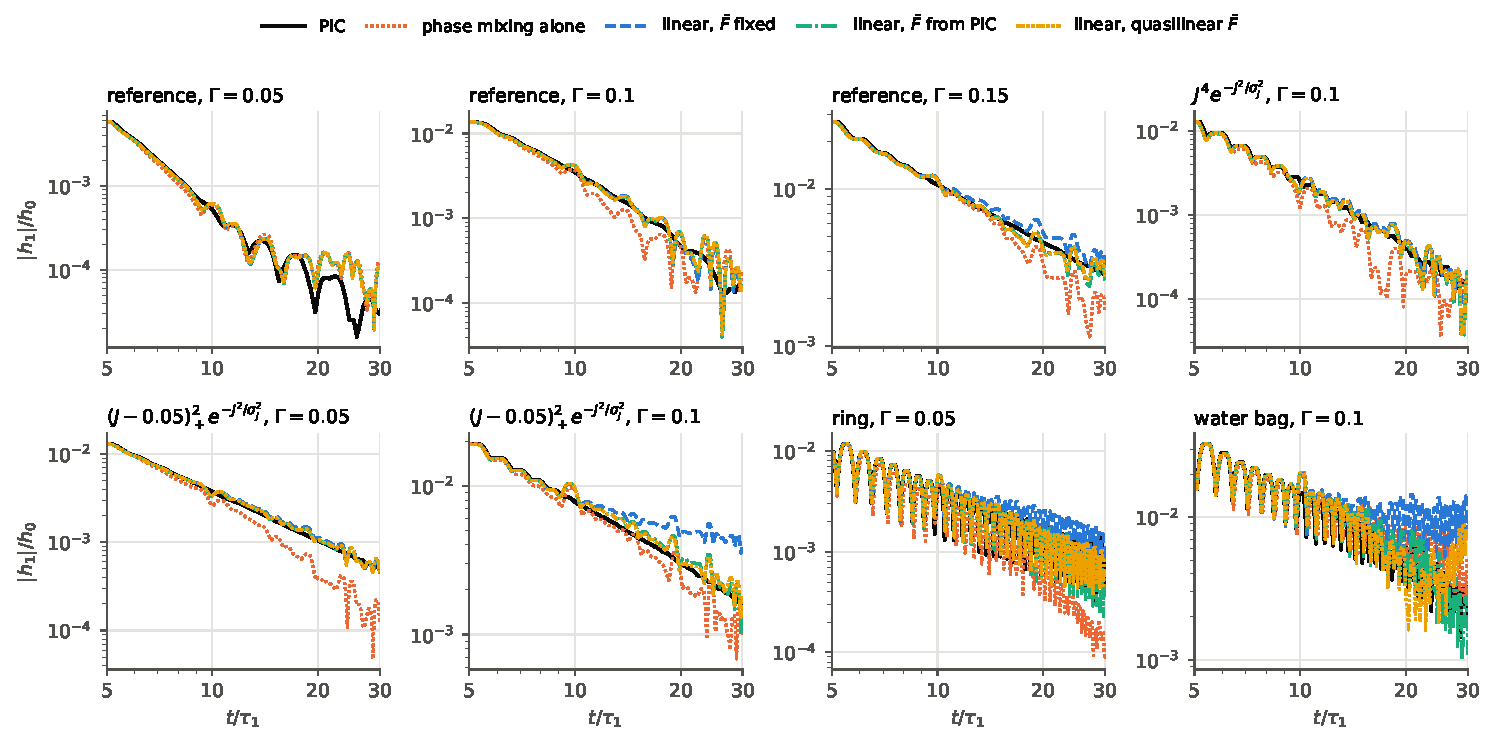
\includegraphics[width=\textwidth]{figuras/respuesta_lineal.pdf}}
\caption{Envelope of $|h_1|/h_0$ from $t_0 = 5\tau_1$ on for eight of the simulations of Table~\ref{Tab:Rates}, computed with the action-angle variables of the averaged potential $\bar{\Phi}$, together with phase mixing alone in $\bar{\Phi}$ and the solutions of Eq.~(\ref{Eq:LinMixed}) with $\bar{F}$ fixed at its value at $t_0$, with $\bar{F}$ replaced by the slow part of the angle average of the DF of the simulation, and with $\bar{F}$ evolved according to the quasilinear equation~(\ref{Eq:Quasilinear}).}
\label{Fig:Response}
\end{figure}

The results are shown in Fig.~\ref{Fig:Response} and Table~\ref{Tab:Response} for eight of the simulations. At $t = 8\tau_1$ and $12\tau_1$ the ratio of $|h_1|$ in the simulation to the one of the solution of Eq.~(\ref{Eq:LinMixed}) lies between $0.85$ and $1.07$ in all of them, and the ratio of the deviations of the potential of the gas from $\bar{\Phi}$ lies between $0.80$ and $1.21$. Phase mixing alone, in contrast, underestimates $|h_1|$ by factors up to $3.3$ at $t = 12\tau_1$ and $3.5$ at $t = 16\tau_1$. Hence, after $t_0$ the slowdown of the mixing is due to the potential of $\delta F$, and it is described by the linear response of the mixed state. In order to locate this response, we compute the difference between $h_1$ of the simulation and phase mixing alone separately for the gas in five overlapping intervals of $J$, defined by triangular weights which are centered at the quantiles $0.02$, $0.25$, $0.5$, $0.75$ and $0.98$ of the distribution of the mass in $J$ and which add up to one. The difference comes from the interval at the inner edge of the support of $\bar{F}$, and for the ring and the water bag also from the one at its outer edge, where $\bar{F}'$ is large; the contributions of the intervals in between are typically smaller by one order of magnitude.

\begin{table}[htp]
\begin{center}
\begin{tabular}{ll|cccc|cccc}
\hline\hline
 & & \multicolumn{4}{c|}{$t = 20\tau_1$} & \multicolumn{4}{c}{$t = 25\tau_1$} \\
dependence on $J$ & $\Gamma$ & mixing & fixed & PIC & quasilinear & mixing & fixed & PIC & quasilinear \\
\hline
\TabRespuesta
\hline\hline
\end{tabular}
\end{center}
\caption{Ratio of the envelope of $|h_1|/h_0$ in the simulation to the one of each approximation at $t = 20\tau_1$ and $t = 25\tau_1$: phase mixing alone in the averaged potential $\bar{\Phi}$, and the solutions of Eq.~(\ref{Eq:LinMixed}) with $\bar{F}$ fixed at its value at $t_0 = 5\tau_1$, with the slow part of the angle average of the DF of the simulation, and with $\bar{F}$ evolved according to Eq.~(\ref{Eq:Quasilinear}). A ratio of one means that the approximation follows the simulation. ``Reference'' is the shape $J^2\exp(-J^2/\sigma_J^2)$ of the cloud~(\ref{Eq:Pulse}).}
\label{Tab:Response}
\end{table}

From $t\approx 16\tau_1$ on, Eq.~(\ref{Eq:LinMixed}) with fixed $\bar{F}$ overestimates $|h_1|$ in the simulations in which $\bar{F}$ has an abrupt edge: at $t = 20\tau_1$ and $25\tau_1$ the ratio of the simulation to the linear solution is $0.66$ and $0.47$ for the shape $(J - 0.05)_+^2\exp(-J^2/\sigma_J^2)$ with $\Gamma = 0.1$, $0.72$ and $0.40$ for the ring, $0.52$ and $0.24$ for the water bag, and $0.87$ and $0.79$ for the reference cloud with $\Gamma = 0.15$, whose DF rises steeply at the circular orbit (Fig.~\ref{Fig:ChangeF}, top row). The linear solution then contains an oscillation of the edge which is damped more slowly than in the simulation (Fig.~\ref{Fig:Response}), and in the interval at the inner edge the response of the simulation differs in phase from the one of the linear solution by $24$ to $35$ degrees at $t = 20\tau_1$.

\begin{figure}[htp]
\centerline{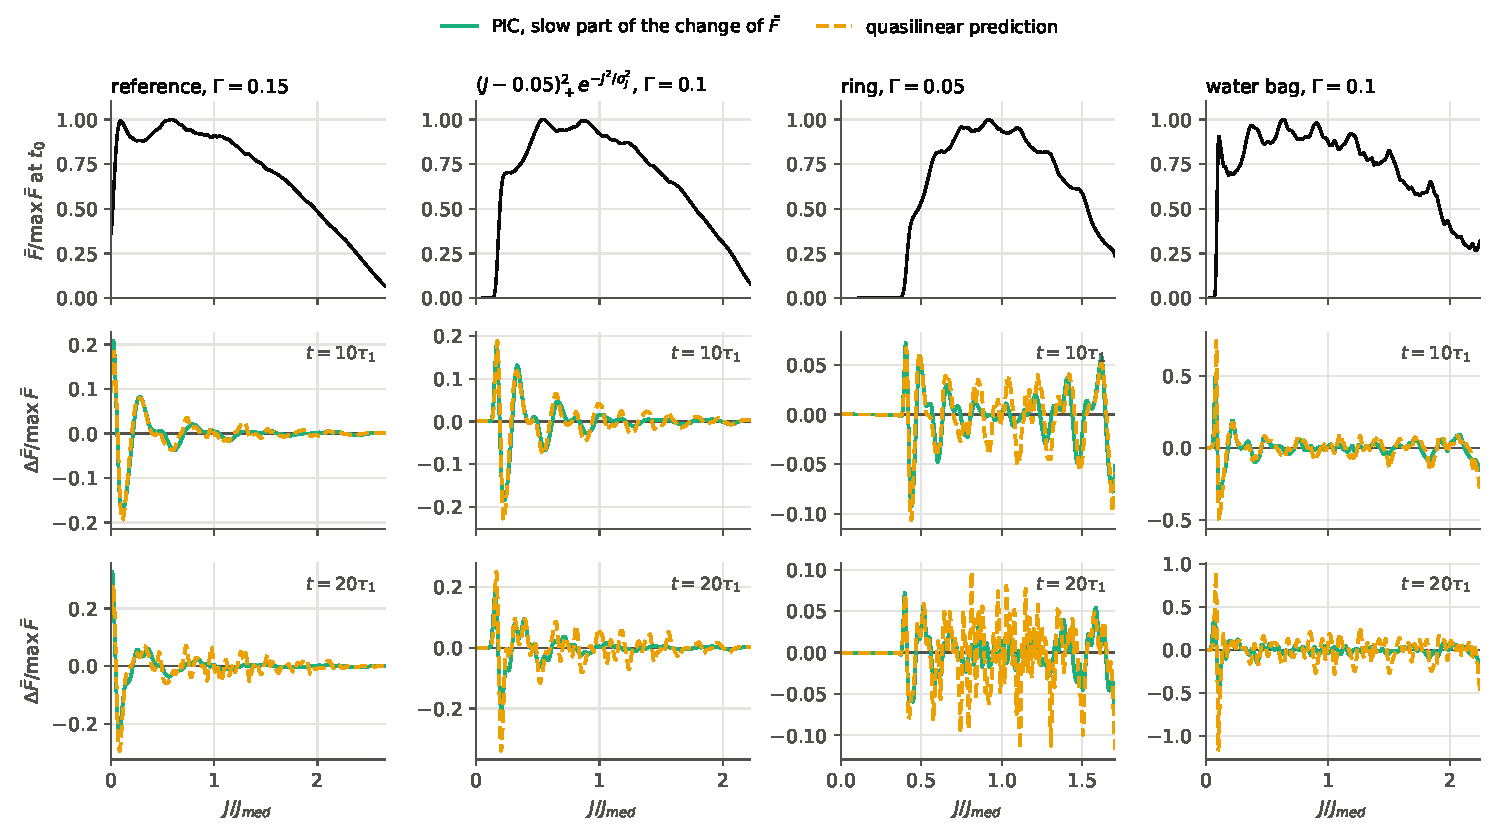
\includegraphics[width=\textwidth]{figuras/cambio_F0.pdf}}
\caption{Top row: angle average $\bar{F}$ of the DF at $t_0 = 5\tau_1$ in units of its maximum, as a function of $J/J_{med}$, for four of the simulations of Fig.~\ref{Fig:Response}. Middle and bottom rows: change of $\bar{F}$ between $t_0$ and $t = 10\tau_1$ and $20\tau_1$, respectively, in the simulation (slow part, averaged over $|t' - t|\leq\tau_1/2$) and according to the quasilinear equation~(\ref{Eq:Quasilinear}). Since the histogram of $J$ inherits the rows of the lattice, all the functions are smoothed with a Gaussian kernel whose width is between $0.007\,J_{med}$ and $0.016\,J_{med}$.}
\label{Fig:ChangeF}
\end{figure}

The reason is that $\bar{F}$ itself changes at these edges after $t_0$. Figure~\ref{Fig:ChangeF} shows the slow part of this change, obtained by averaging the angle average of the DF of the simulation, computed with the variables of $\bar{\Phi}$, over the interval $|t' - t|\leq\tau_1/2$. The abrupt edges are smoothed: $\bar{F}$ increases on the side of the edge where it is small and decreases on the other side. At $t = 20\tau_1$ the change reaches $0.33$ of the maximum of $\bar{F}$ at the circular orbit for the reference cloud with $\Gamma = 0.15$, and $0.20$, $0.07$ and $0.49$ of it at the inner edge for the shape $(J - 0.05)_+^2\exp(-J^2/\sigma_J^2)$ with $\Gamma = 0.1$, for the ring and for the water bag, respectively. When $\bar{F}'$ in Eq.~(\ref{Eq:LinMixed}) is replaced, at each time, by the derivative of this slow part, the ratios at $t = 20\tau_1$ and $25\tau_1$ become $1.01$ and $0.91$, $1.02$ and $1.46$, $1.25$ and $0.51$, and $1.08$ and $1.00$, respectively, see Table~\ref{Tab:Response}; at $t = 25\tau_1$ the ring passes through a minimum of $|h_1|$, at which the ratio is not meaningful. The curves follow the simulations up to $t = 30\tau_1$, except for the water bag, for which they deviate by up to a factor of two after $t\approx 20\tau_1$, and the difference of phase at the inner edge is reduced to between $5$ and $22$ degrees at $t = 20\tau_1$. The change of the potential after $t_0$ plays no role: the orbital frequencies in the potentials averaged over intervals of length $\tau_1$ differ so little from $\bar{\Omega}$ that, in all eight simulations, the dispersion of the phase which they accumulate up to $t = 30\tau_1$, weighted with $\bar{F}$, is at most $0.015$ radians.

The change of $\bar{F}$ is of second order in $\delta F$, and it can be computed without using the simulation after $t_0$. Averaging the Vlasov equation in the variables $(Q,J)$ of $\bar{\Phi}$ over $Q$ gives
\begin{equation}
\frac{\partial\bar{F}}{\partial t} = \frac{\partial}{\partial J}\langle\delta F\,\frac{\partial\delta\Phi}{\partial Q}\rangle,
\label{Eq:Quasilinear}
\end{equation}
where $\langle\cdot\rangle$ denotes the average over $Q$. We have integrated this equation together with Eq.~(\ref{Eq:LinMixed}), with $\delta F$ and $\delta\Phi$ given by the linear solution, and replaced $\bar{F}'$ in Eq.~(\ref{Eq:LinMixed}) by the derivative of the result, which is the quasilinear approximation of plasma physics.\EJ{Reference for the quasilinear approximation to be added, after checking it (Vedenov, Velikhov and Sagdeev 1961; Drummond and Pines 1962).} The change of $\bar{F}$ which is obtained in this way agrees with the one of the simulation up to $t\approx 12\tau_1$: for the four simulations of Fig.~\ref{Fig:ChangeF} the correlation coefficient between the two functions of $J$ lies between $0.81$ and $0.98$ at $t = 8\tau_1$ and $12\tau_1$, and at $t = 8\tau_1$ their largest values agree to within $23$ percent. Later the two changes depart from each other: at $t = 20\tau_1$ the ratio of their largest values, quasilinear to simulated, lies between $0.88$ and $2.4$, and the quasilinear change develops oscillations in $J$ (Fig.~\ref{Fig:ChangeF}, bottom row). Nevertheless, the linear solution with the quasilinear $\bar{F}$ gives the ratios $1.08$ and $0.86$, $1.06$ and $1.54$, $2.14$ and $0.68$, and $1.12$ and $0.98$ at $t = 20\tau_1$ and $25\tau_1$ for the four simulations, which are close to those obtained with the $\bar{F}$ of the simulation, except for the water bag, for which the response of the two edges is damped too strongly. This is consistent with the faster decay of $|h_1|$ for the water bag with self-gravity than without it (section~\ref{SubSec:RatesDecay}): its abrupt edges, which are responsible for the tail $t^{-1}$, are smoothed.

In two of the simulations the late evolution is not described by any of these approximations. For the reference cloud with $\Gamma = 0.05$ and $0.1$, the simulation departs from all the curves of Fig.~\ref{Fig:Response}, including phase mixing alone, from $t\approx 16\tau_1$ and $20\tau_1$ on, respectively, when $|h_1|/h_0$ has decayed to $1.1\times 10^{-4}$ and $4.7\times 10^{-4}$. In these two simulations $\bar{F}$ changes by at most five percent of its maximum, and the difference between the simulation and the linear solution comes from the bulk of the support, where the linear response is small.\EJ{Unexplained, and noted as pending (18 November 2026). A possible cause is a floor of about $10^{-4}$ in the reconstruction of $h_1$ with the variables of $\bar{\Phi}$, already seen in a control with $\Gamma = 0.05$; it has not been checked.}

In summary, self-gravity changes the mixing of the clouds which relax in two ways. While the cloud is compact, its potential transports gas towards the circular orbit and lowers the regularity of the DF at the inner edge of its support, which sets a slower tail according to Eq.~(\ref{Eq:Tail}). Afterwards, the potential of the part of the DF which is not yet mixed acts on the mixed state, whose linear response is concentrated at the edges of its support and slows down the mixing further. This response is damped as the mixed state smooths its abrupt edges, a process which is described by Eq.~(\ref{Eq:Quasilinear}) up to $t\approx 12\tau_1$. Throughout, the potential of the gas approaches a stationary profile at a rate comparable to the one of the mixing.
